\section{Data Category and Language Distribution Statistics}
\label{appendix:a}

We prompt \texttt{Claude Sonnet 4} to generate 20 language-agnostic category labels for classification:

\begin{itemize}
  \item \textbf{Core Programming Concepts}: \textit{Language Fundamentals}, \textit{Functions \& Modules}, \textit{Object-Oriented Programming}, \textit{Functional Programming}, \textit{Memory Management \& Performance}, \textit{Error Handling \& Debugging}
  
  \item \textbf{Data and Algorithms}: \textit{Data Structures \& Collections}, \textit{Algorithms \& Problem Solving}, \textit{String \& Text Processing}, \textit{File \& I/O Operations}, \textit{Concurrency \& Async Programming}
  
  \item \textbf{Application Domains}: \textit{Network Programming \& Communication}, \textit{Database Operations \& Persistence}, \textit{Web Development \& Frameworks}, \textit{Mobile \& Cross-platform Development}, \textit{Systems Programming \& Low-level Development}
  
  \item \textbf{Advanced Topics and Tooling}: \textit{Data Science \& Analytics}, \textit{Machine Learning \& AI}, \textit{Testing \& Quality Assurance}, \textit{Development Tools \& Ecosystem}
\end{itemize}



\begin{figure}[t]
\centering
\begin{subfigure}[b]{0.24\textwidth}
    \centering
    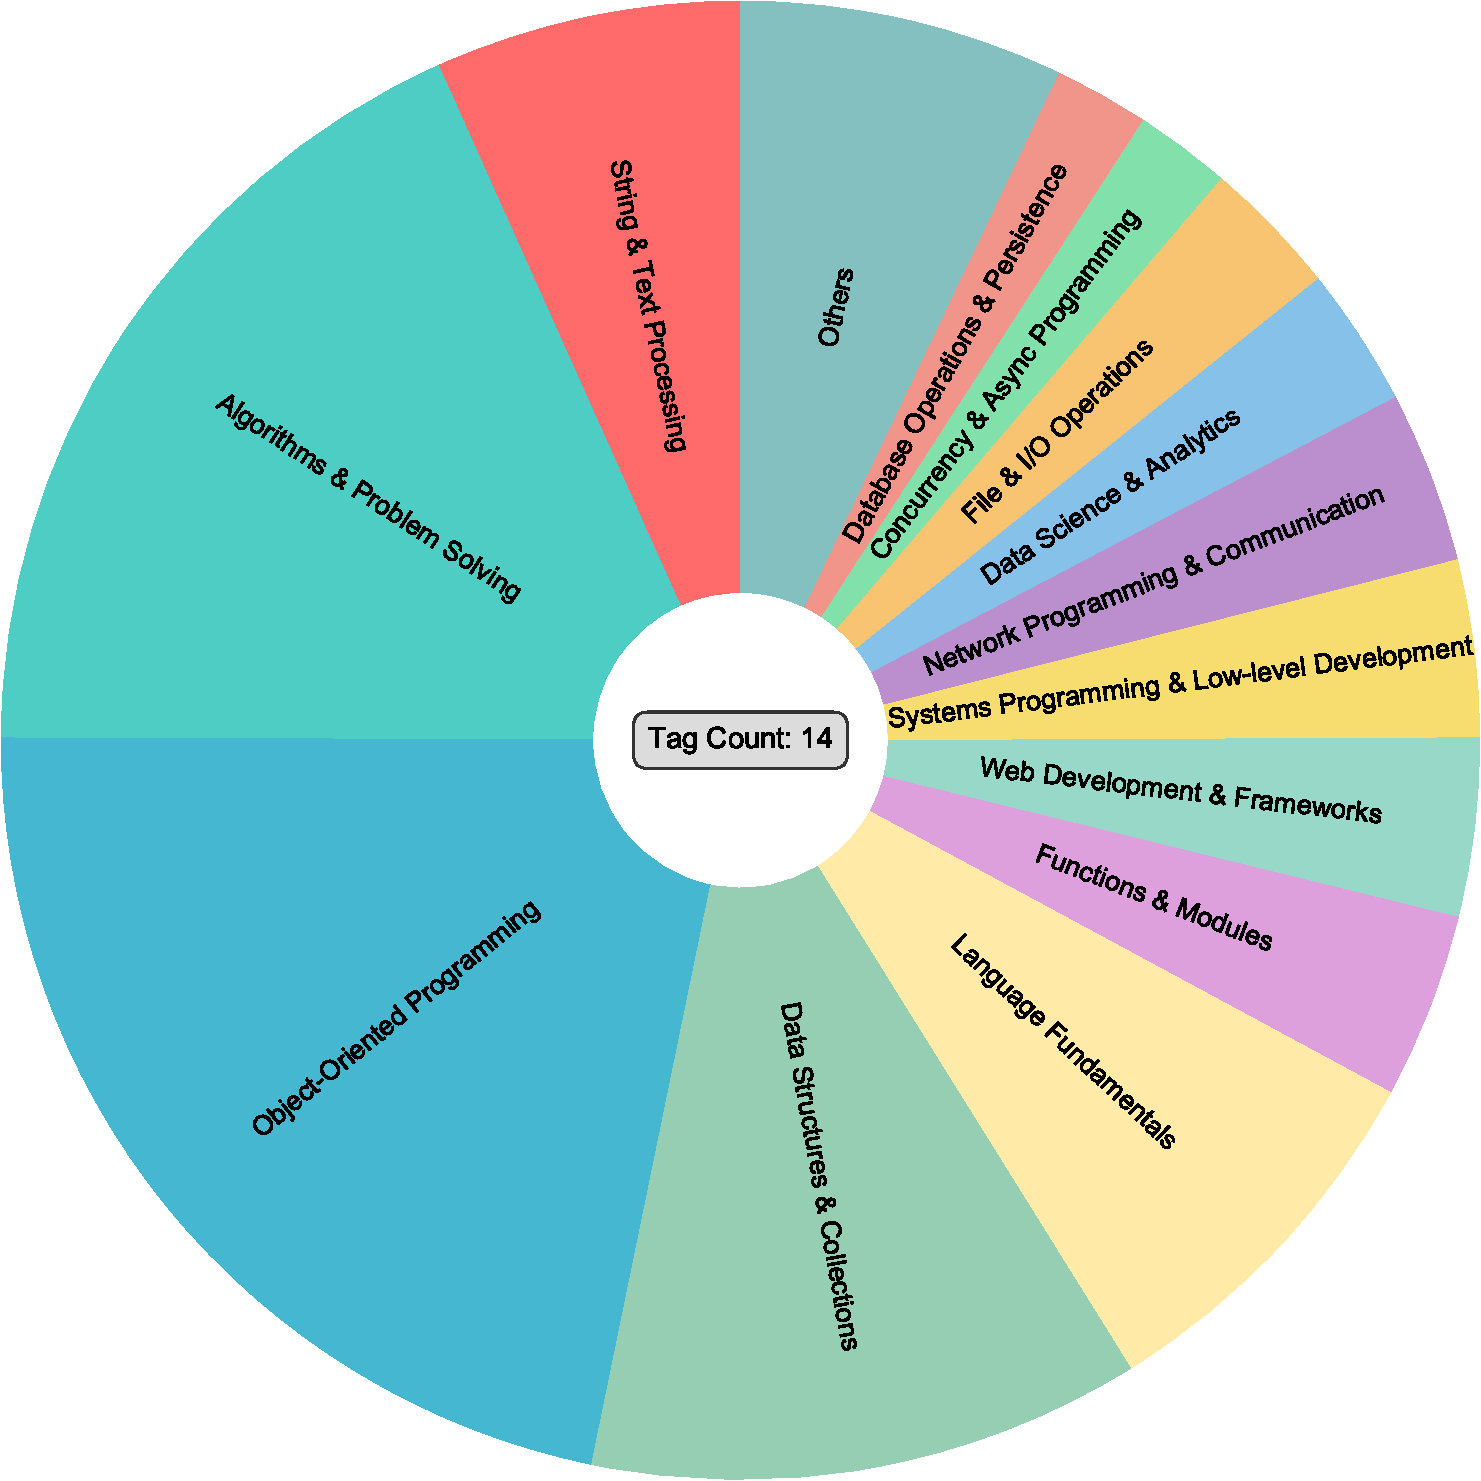
\includegraphics[width=\textwidth]{figures/tag_acb.pdf}
    \caption{AutoCodeBench}
\end{subfigure}
\hfill
\begin{subfigure}[b]{0.24\textwidth}
    \centering
    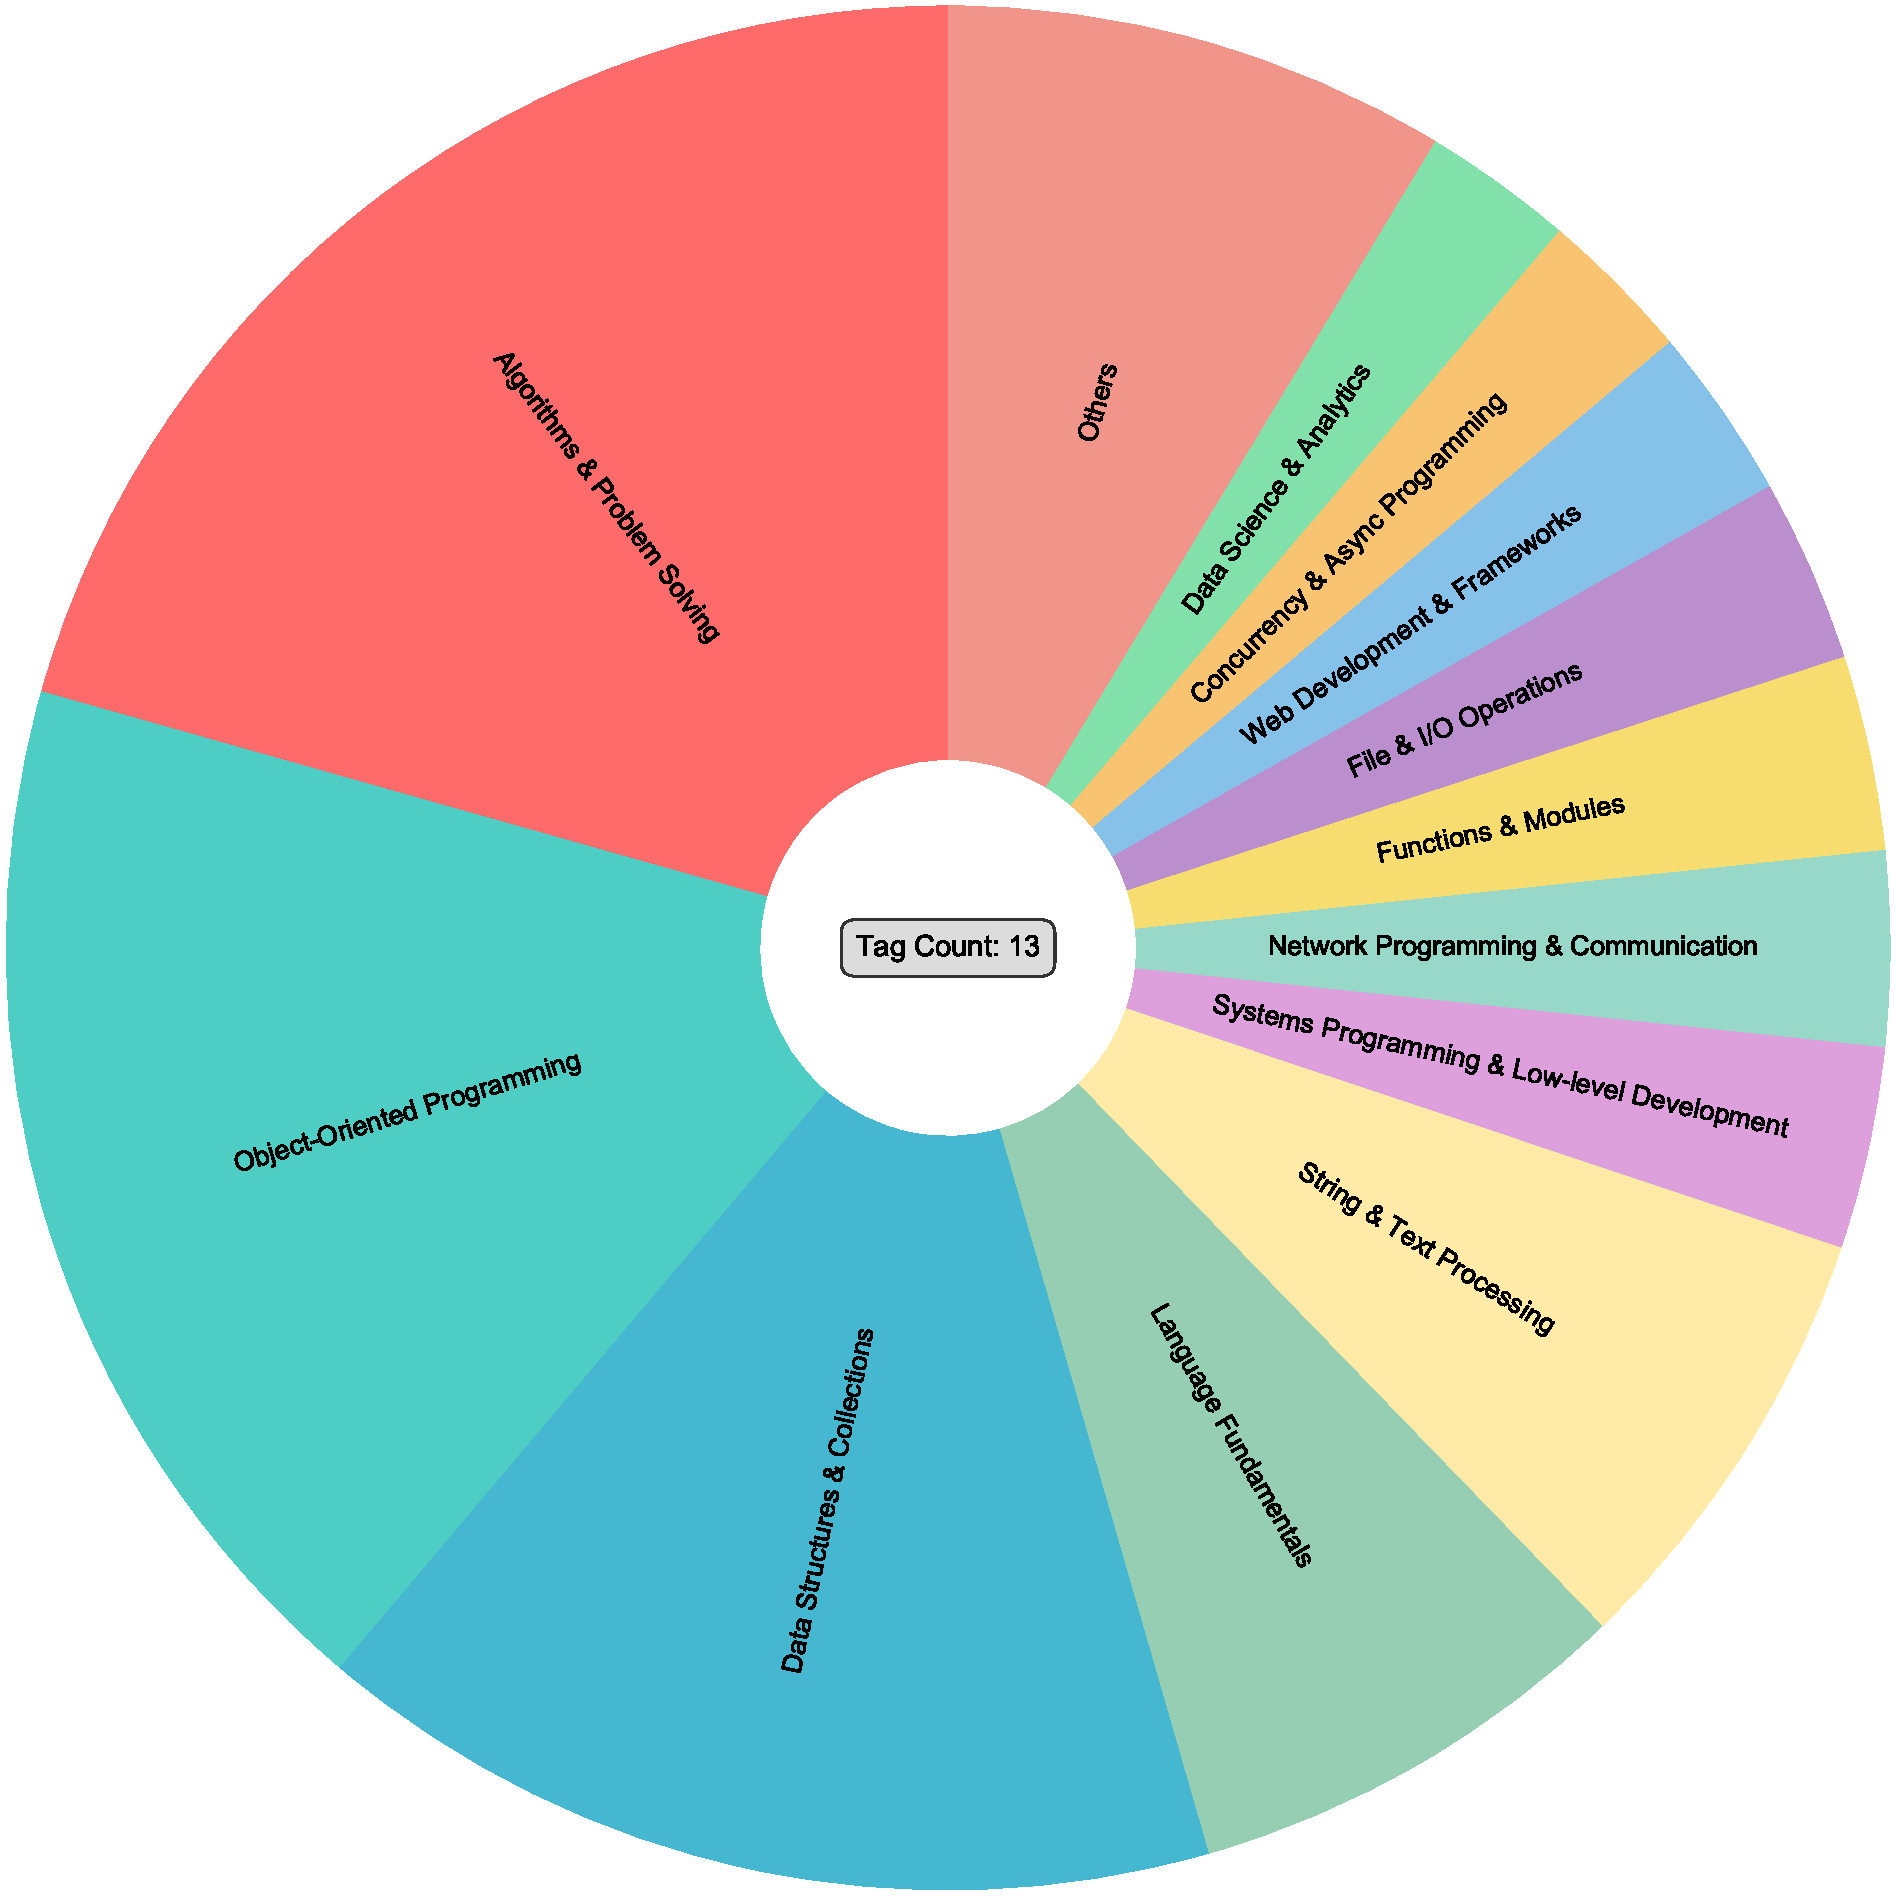
\includegraphics[width=\textwidth]{figures/tag_acb-lite.pdf}
    \caption{AutoCodeBench-Lite}
\end{subfigure}
\hfill
\begin{subfigure}[b]{0.24\textwidth}
    \centering
    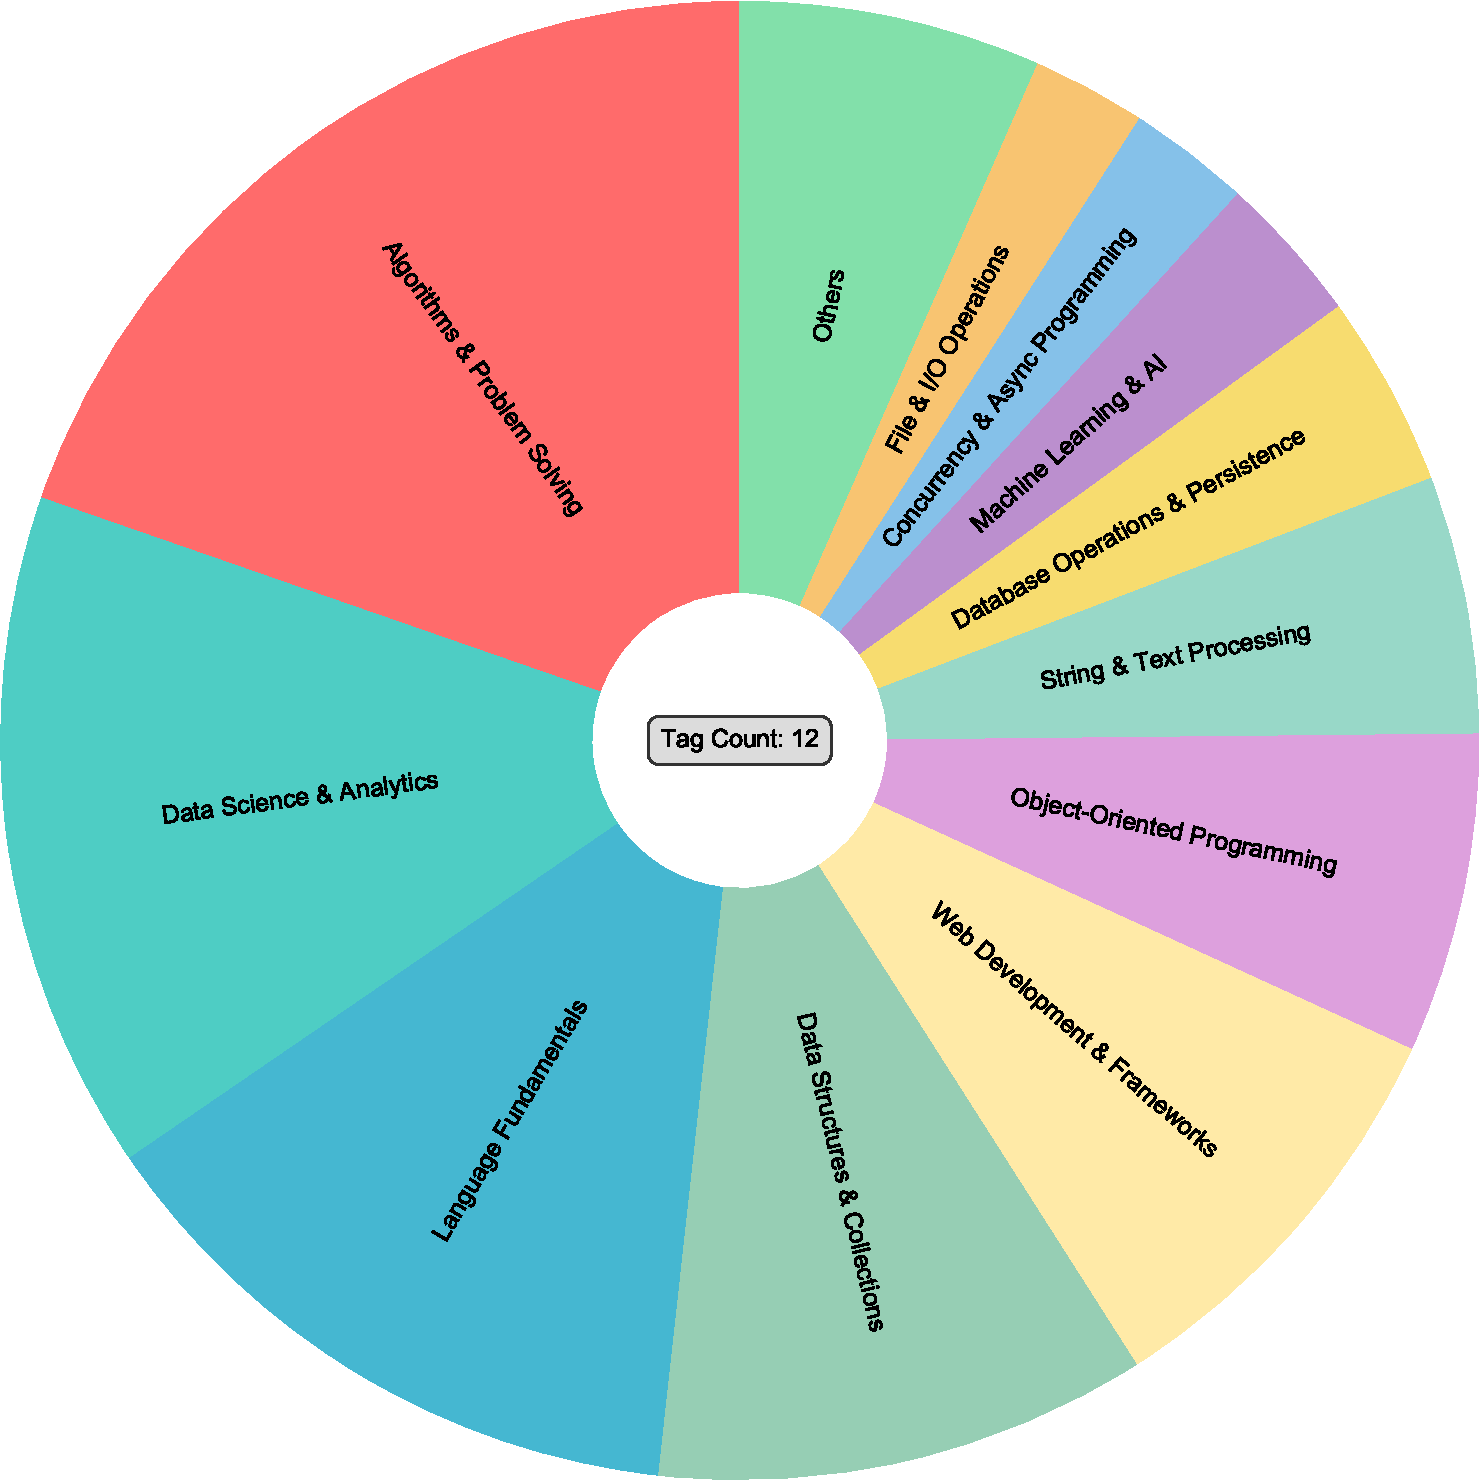
\includegraphics[width=\textwidth]{figures/tag_fsb.pdf}
    \caption{FullStackBench}
\end{subfigure}
\hfill
\begin{subfigure}[b]{0.24\textwidth}
    \centering
    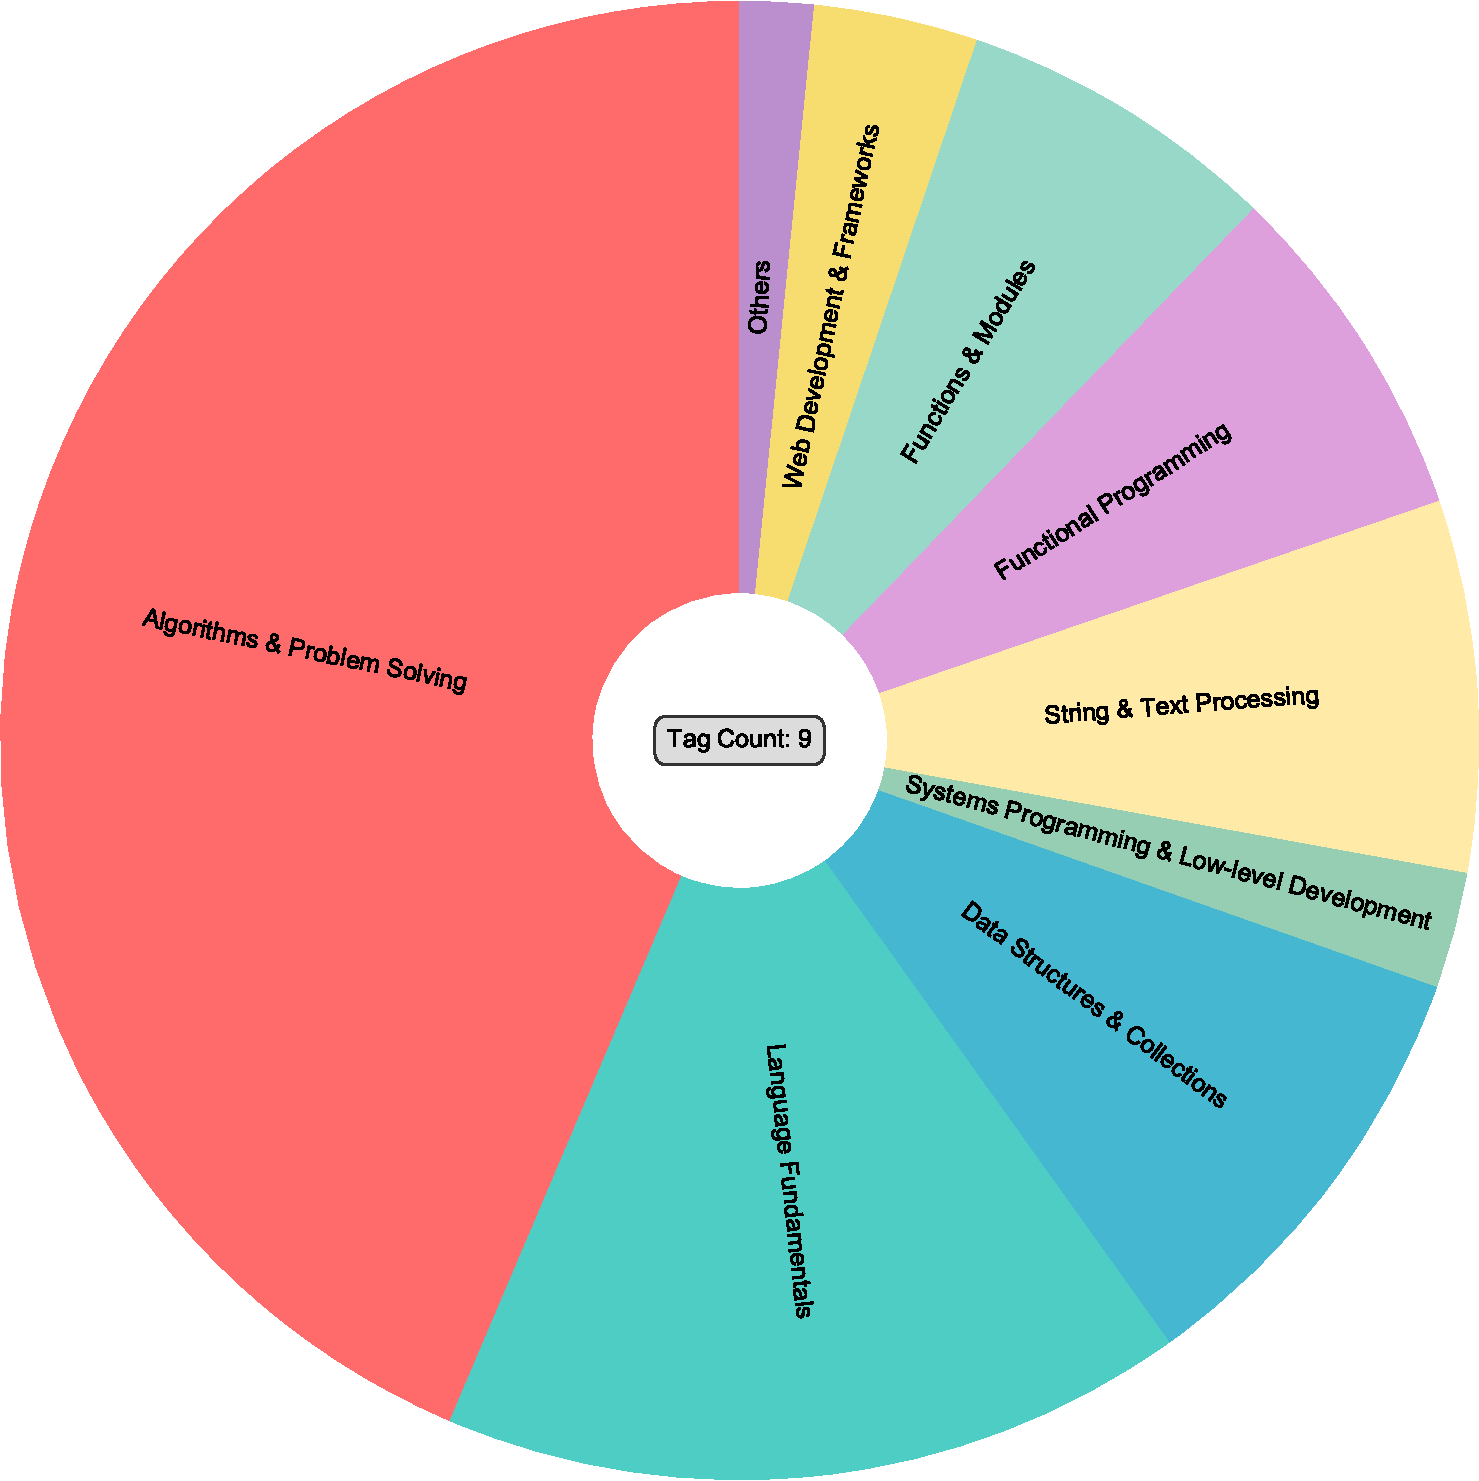
\includegraphics[width=\textwidth]{figures/tag_mceval.pdf}
    \caption{McEval}
\end{subfigure}


\caption{Category Distribution of Different Benchmarks.}
\label{appendix:tag}
\end{figure}



\begin{figure}[t]
\centering
\begin{subfigure}[b]{0.24\textwidth}
    \centering
    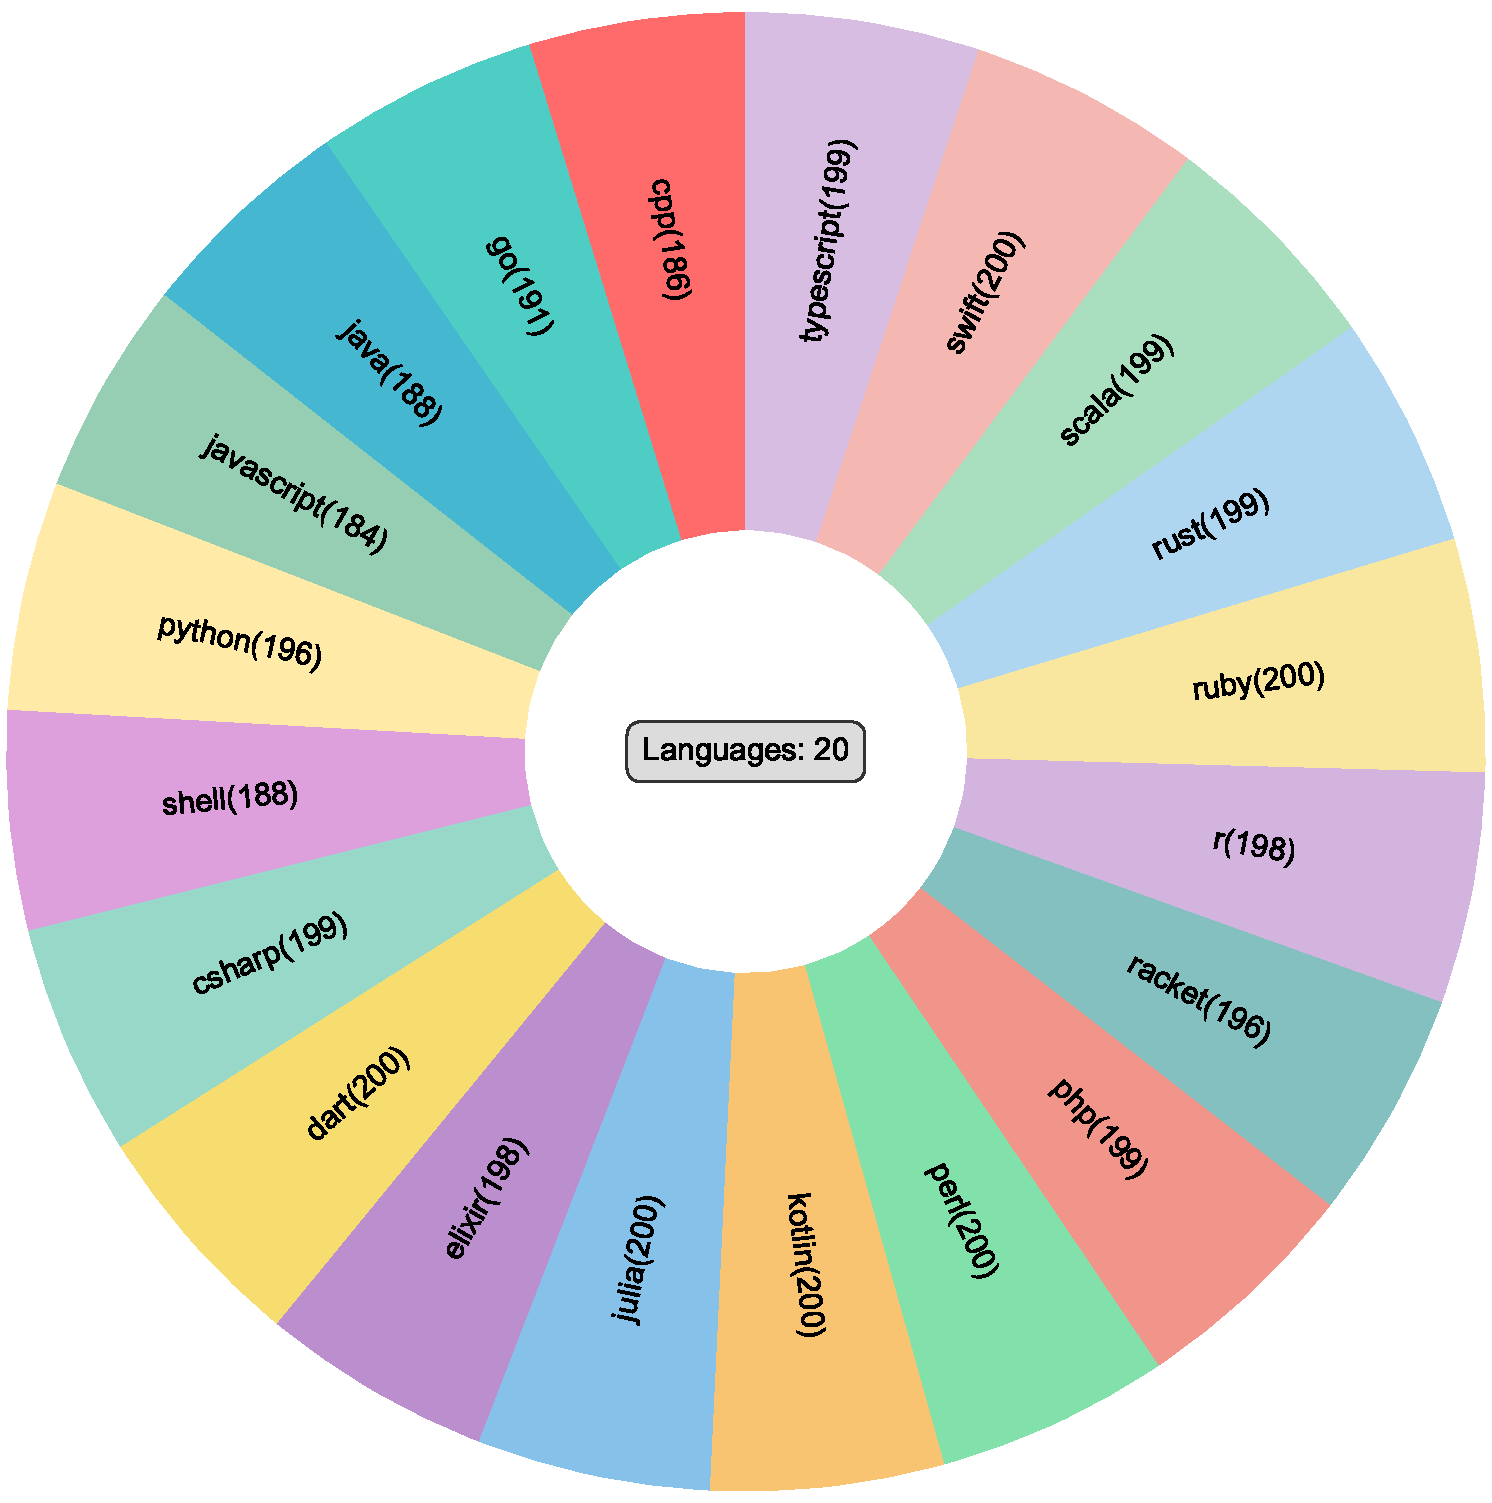
\includegraphics[width=\textwidth]{figures/lan_acb.pdf}
    \caption{AutoCodeBench}
\end{subfigure}
\hfill
\begin{subfigure}[b]{0.24\textwidth}
    \centering
    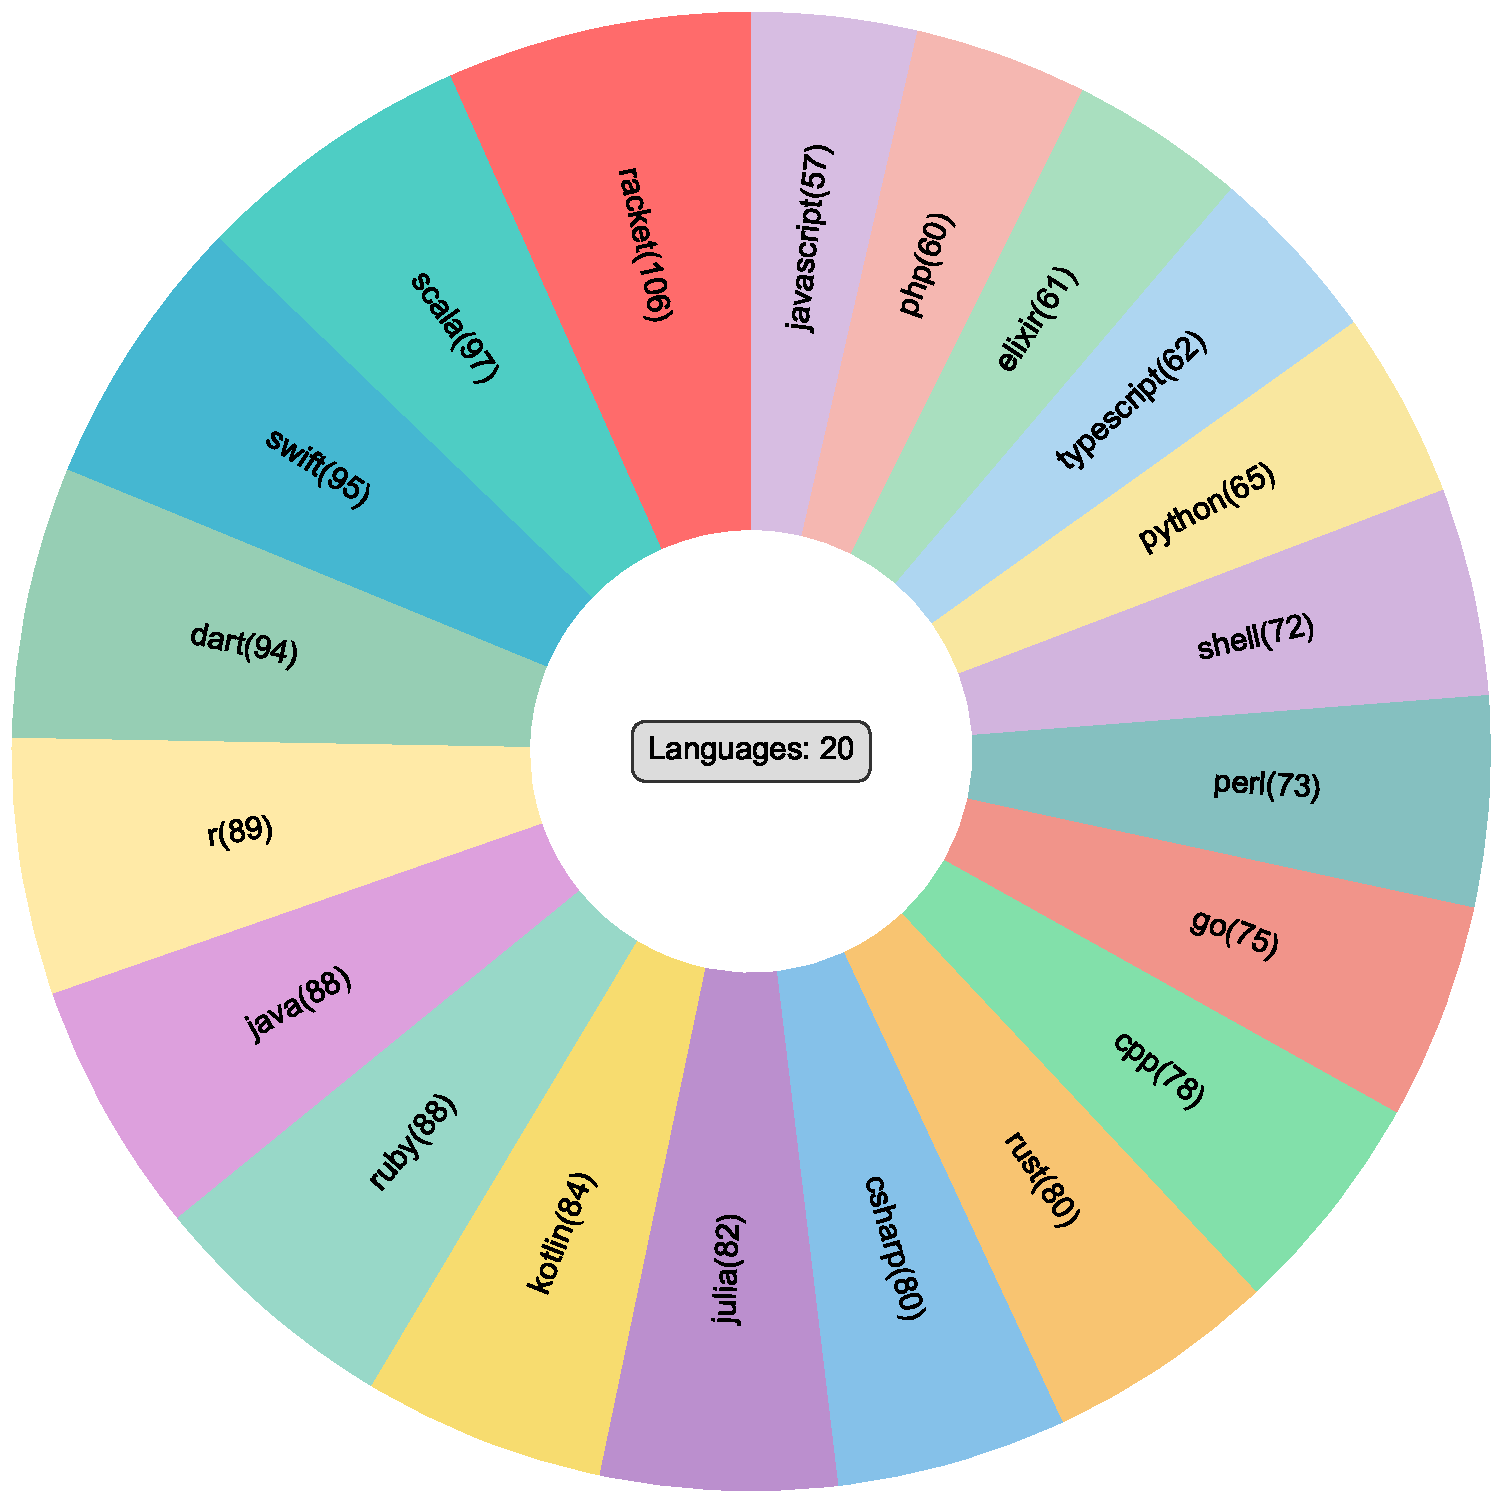
\includegraphics[width=\textwidth]{figures/lan_acb-lite.pdf}
    \caption{AutoCodeBench-Lite}
\end{subfigure}
\hfill
\begin{subfigure}[b]{0.24\textwidth}
    \centering
    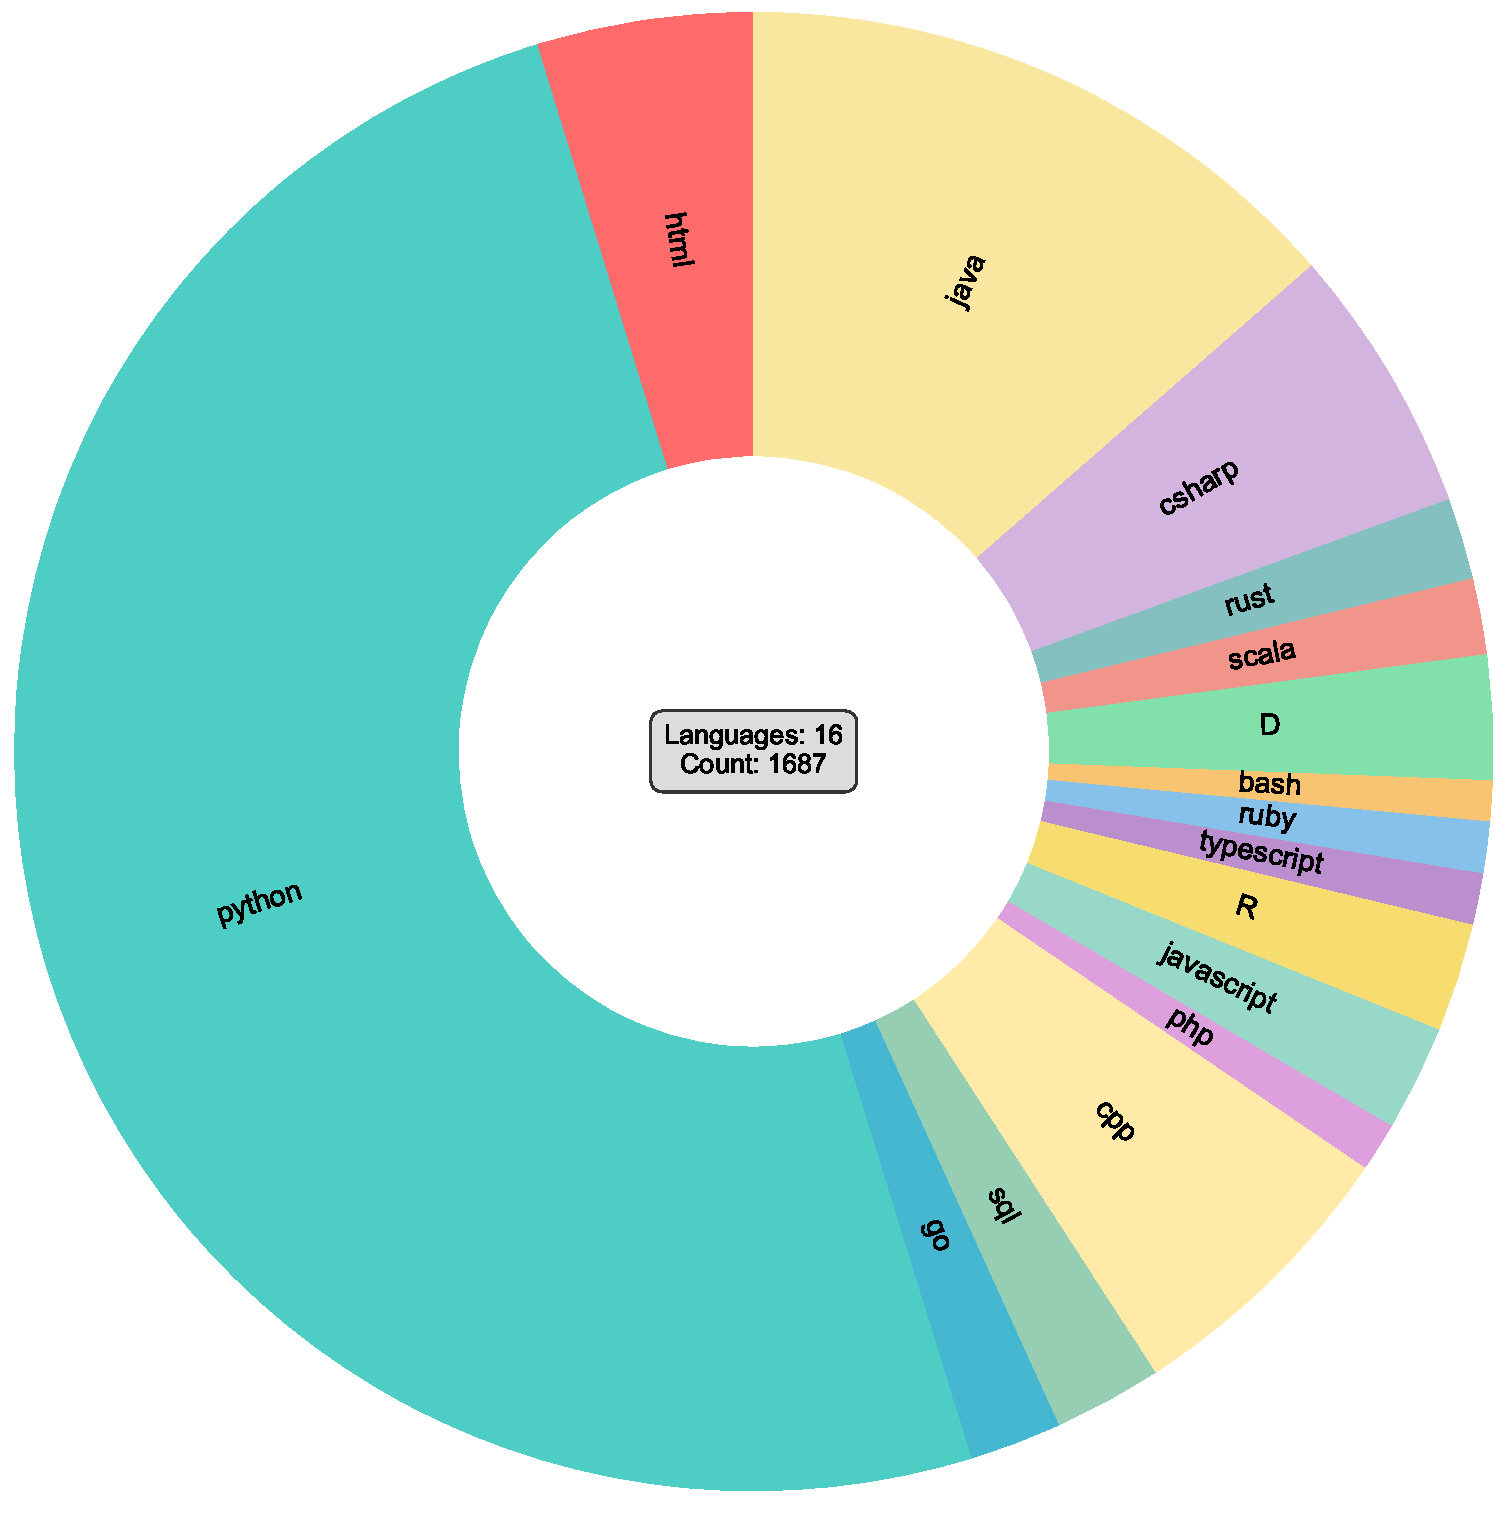
\includegraphics[width=\textwidth]{figures/lan_fsb.pdf}
    \caption{FullStackBench}
\end{subfigure}
\hfill
\begin{subfigure}[b]{0.24\textwidth}
    \centering
    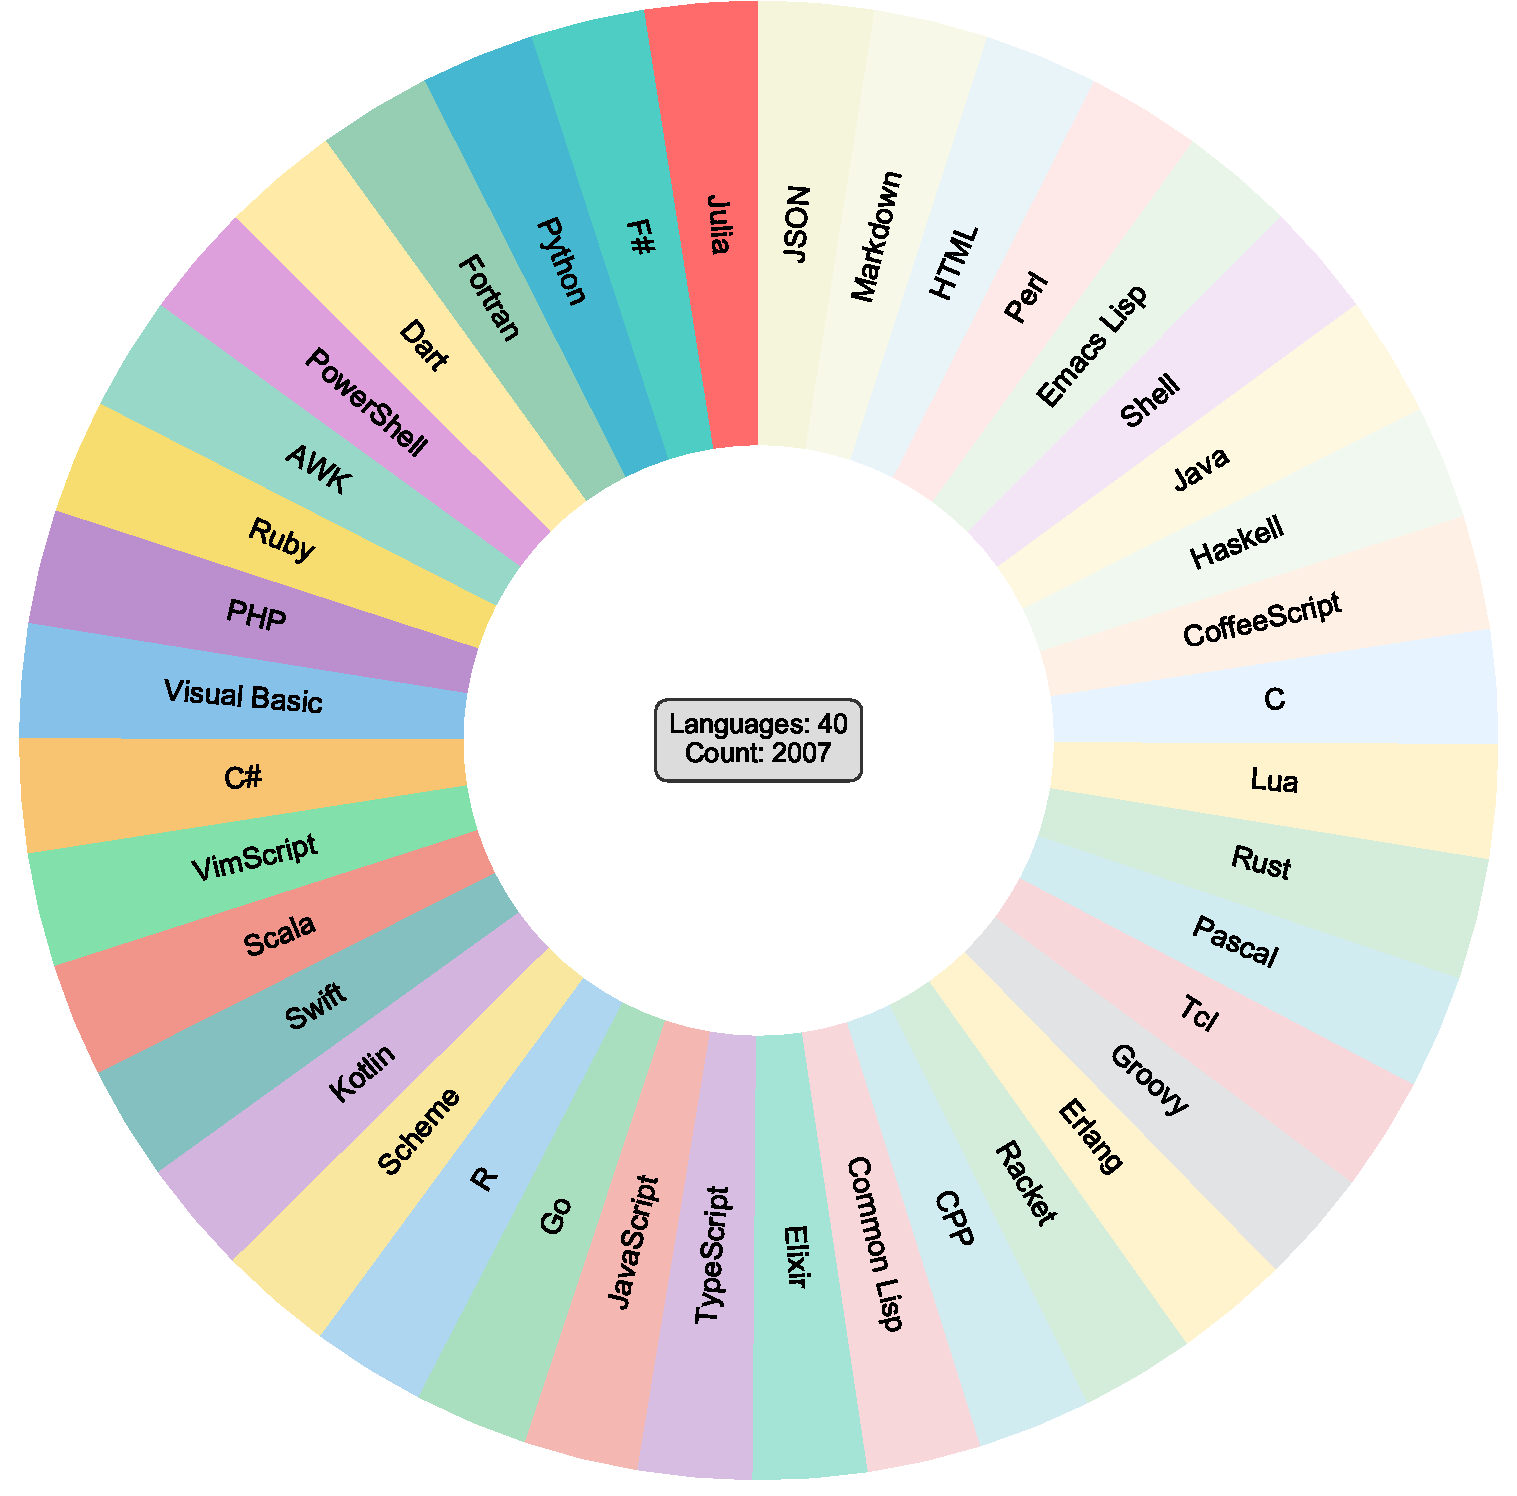
\includegraphics[width=\textwidth]{figures/lan_mceval.pdf}
    \caption{McEval}
\end{subfigure}

\caption{Language Distribution of Different Benchmarks.}
\label{appendix:lan}
\end{figure}



In addition to AutoCodeBench, we conduct task tagging and language distribution analysis for AutoCodeBench-Lite, FullStackBench, and McEval. The results are presented in Figures~\ref{appendix:tag} and~\ref{appendix:lan}. FullStackBench demonstrates comparable category diversity to AutoCodeBench(-Lite) but suffers from an imbalanced language distribution. In contrast, McEval exhibits a well-balanced multilingual distribution but lacks diversity and balance in its category coverage. Our AutoCodeBench(-Lite) achieves the most comprehensive category coverage while maintaining a balanced multilingual distribution, enabling thorough and accurate evaluation of LLMs' multilingual code generation capabilities.



\section{Manual Verification}
\label{appendix:b}


\begin{table}[t]
\small
\begin{tabular}{lccccccc}
\toprule
                    & \textbf{Average}  & \textbf{Python} & \textbf{C++} & \textbf{Java} & \textbf{JS} & \textbf{Go} & \textbf{Shell} \\
                    \midrule
Problem Accuracy    & 87.6 & 83.5            & 88.0           & 86.0            & 89.0          & 86.0          & 93.3           \\
\midrule
Current Upper Bound & 66.9\textcolor{red}{$_{\Delta20.7}$} & 61.7\textcolor{red}{$_{\Delta21.8}$}            & 71.5\textcolor{red}{$_{\Delta16.5}$}         & 76.1\textcolor{red}{$_{\Delta9.9}$}          & 58.2\textcolor{red}{$_{\Delta30.8}$}        & 65.4\textcolor{red}{$_{\Delta20.6}$}        & 68.6\textcolor{red}{$_{\Delta24.7}$}           \\
\midrule
Claude 4 Opus (Reasoning)    & 44.6\textcolor{red}{$_{\Delta43.0}$} & 40.3\textcolor{red}{$_{\Delta43.2}$}            & 44.1\textcolor{red}{$_{\Delta43.9}$}         & 55.9\textcolor{red}{$_{\Delta30.1}$}          & 38.6\textcolor{red}{$_{\Delta50.4}$}        & 37.2\textcolor{red}{$_{\Delta48.8}$}        & 51.6\textcolor{red}{$_{\Delta41.7}$}   \\
\bottomrule
\end{tabular}
\caption{Comparison of Accuracy, Upper Bound, and Model Performance.}
\label{appendix:accuracy}
\end{table}





Due to the involvement of multiple languages and domains in the data, directly verifying the quality of the data through manual annotation presents significant challenges. To address this issue, we employ a Human-LLM collaboration approach for data quality validation. Specifically, we design prompts in the native languages of the annotators and use the \texttt{DeepSeek-R1-0528} to generate detailed reasoning processes and checklist-based annotation results. The prompt is shown in Figure~\ref{appendix:prompt_annotation}. During the annotation process, we assume that the programming problems are completely correct. The primary task of the annotators is to assess the correctness of the test functions and their alignment with the programming problem, based on the LLM's output. We allow for test cases that may not cover all boundary conditions, focusing primarily on the correctness of the test functions rather than their comprehensiveness. The annotators pay particular attention to the following aspects:
\begin{itemize}
    \item Whether the function names, class names, variable definitions, and return types are consistent with the problem description;
    \item Whether the test cases exhibit randomness or non-reproducibility;
    \item Whether the test cases contradict the logic presented in the problem statement;
    \item Whether there are any precision issues with the test cases;
    \item Whether the test functions include test cases that are not addressed in the problem description.
\end{itemize}




% \begin{figure}[t]
% \centering
% \includegraphics[width=0.9\textwidth]{figures/annotation.png}
% \caption{The front-end interface for annotation.}
% \label{appendix:annotation}
% \end{figure}


\begin{figure}[t]
\centering
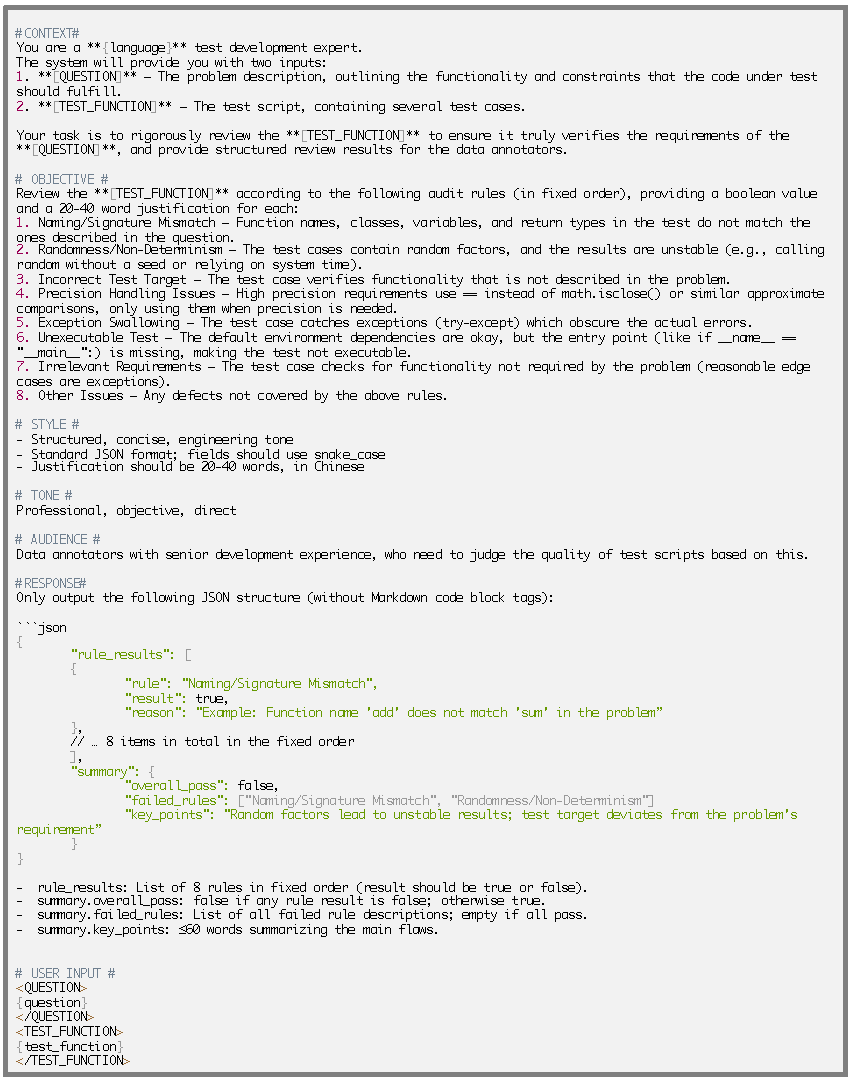
\includegraphics[width=0.9\textwidth]{figures/prompt_annotation.pdf}
\caption{The English prompt of annotation and critic.}
\label{appendix:prompt_annotation}
\end{figure}



To facilitate annotation, we design a front-end interface, including question, test function, critic reasoning process and results from LLM. Based on the information provided in the interface, the annotators generate a binary classification output.

Using the annotation results, we calculate the problem accuracy rates for different programming languages (Python, C++, Java, JavaScript, Go, Shell), as shown in Table~\ref{appendix:accuracy}. The results indicate that, despite the presence of some noisy data, our benchmark model still demonstrates high accuracy (87.6\%). Furthermore, even after removing the noise, the current SOTA model shows significant room for improvement ($\Delta43.0$), further validating the high difficulty level of our benchmark. Besides, we find that, compared to logic errors in the problem description and errors in the test functions, the most frequently occurring issue is \textbf{incomplete problem descriptions}. For example, some test functions reference class or function names that are essential but not explicitly mentioned in the problem description, or they require natural language outputs for edge cases that are not explicitly specified in the problem statement, leading to mismatches between the generated code and the test functions. Interestingly, we observe similar issues in manually annotated BigCodeBench~\citep{zhuo2025bigcodebench}, highlighting the significant challenge of creating comprehensive and accurate programming problems for annotators.





\begin{figure*}[t]
    \centering
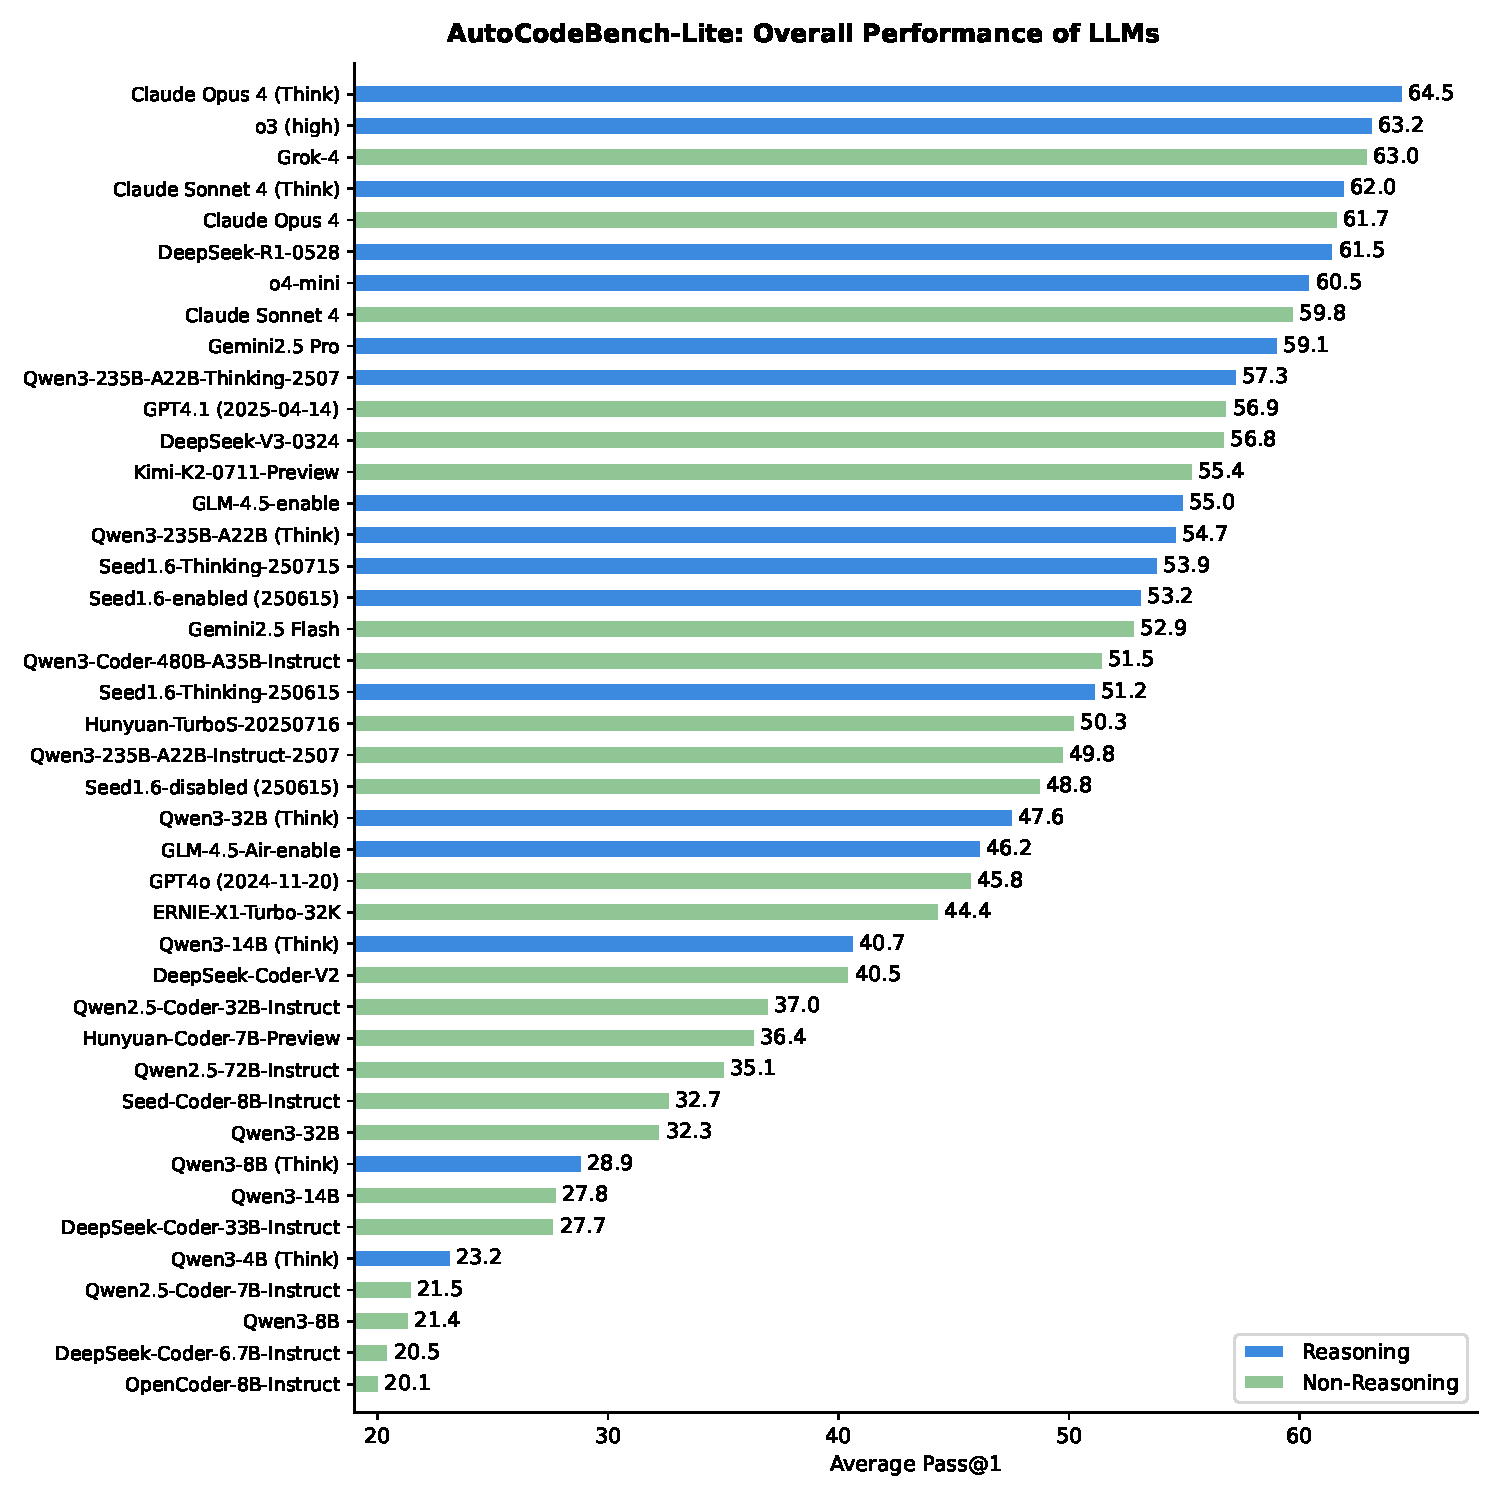
\includegraphics[width=1.0\columnwidth]{figures/leaderboard_lite.pdf}
    \caption{AutoCodeBench-Lite leaderboard showing Pass@1 performance of various LLMs.}
	\label{appendix:leaderboard_lite}
\end{figure*}




\section{Multilingual Code Sandbox Service}

This service offers a secure and high-performance environment for the compilation and execution of code in over 30 programming languages. It supports large-scale code data validation, making it suitable for high-volume, automated testing scenarios. Our multilingual sandbox has the following features:

\begin{itemize}
    \item \textbf{Multilingual Support}: The service supports more than 30 programming languages, including popular ones like Python, JavaScript, Go, Java, C++, and Rust, providing versatility for various use cases.
    \item \textbf{Security Isolation}: Code execution is isolated within Docker containers, ensuring that each execution environment is separate. Additionally, iptables firewall rules are applied to maintain a high level of security, preventing unauthorized access or interference.
    \item \textbf{Smart Code Integration}: The system automatically manages the integration of function code with testing code. It adapts to language-specific syntax, ensuring seamless execution without requiring manual intervention for code merging.
    \item \textbf{High Performance}: Powered by a Gunicorn multi-process architecture, the sandbox supports concurrent execution of multiple code instances, making it capable of handling a high volume of requests efficiently.
    \item \textbf{RESTful API}: The service provides a clean and easy-to-use HTTP-based API, allowing developers to interact with the sandbox programmatically, whether for integrating into larger applications or automating tasks.
    \item \textbf{Extensive Language Support}: Beyond the mainstream languages, the sandbox also supports emerging and niche languages, allowing it to cater to a wide variety of development environments and user needs.
    \item \textbf{Custom Execution Environments}: Users can configure specific environments for their tasks, enabling tailored execution conditions based on their unique requirements.
\end{itemize}







\section{Prompts for Automated Workflow}

The prompt of generating code solution is shown in Figure~\ref{appendix:prompt_solution}.

The prompt of generating test function is shown in Figure~\ref{appendix:prompt_test}.

The prompt of generating programming problem is shown in Figure~\ref{appendix:prompt_problem}.

The prompt of LLM-as-Critic is shown in Figure~\ref{appendix:prompt_annotation}.

The prompt of translating languages is shown in Figure~\ref{appendix:prompt_translate}.




\begin{figure}[t]
\centering
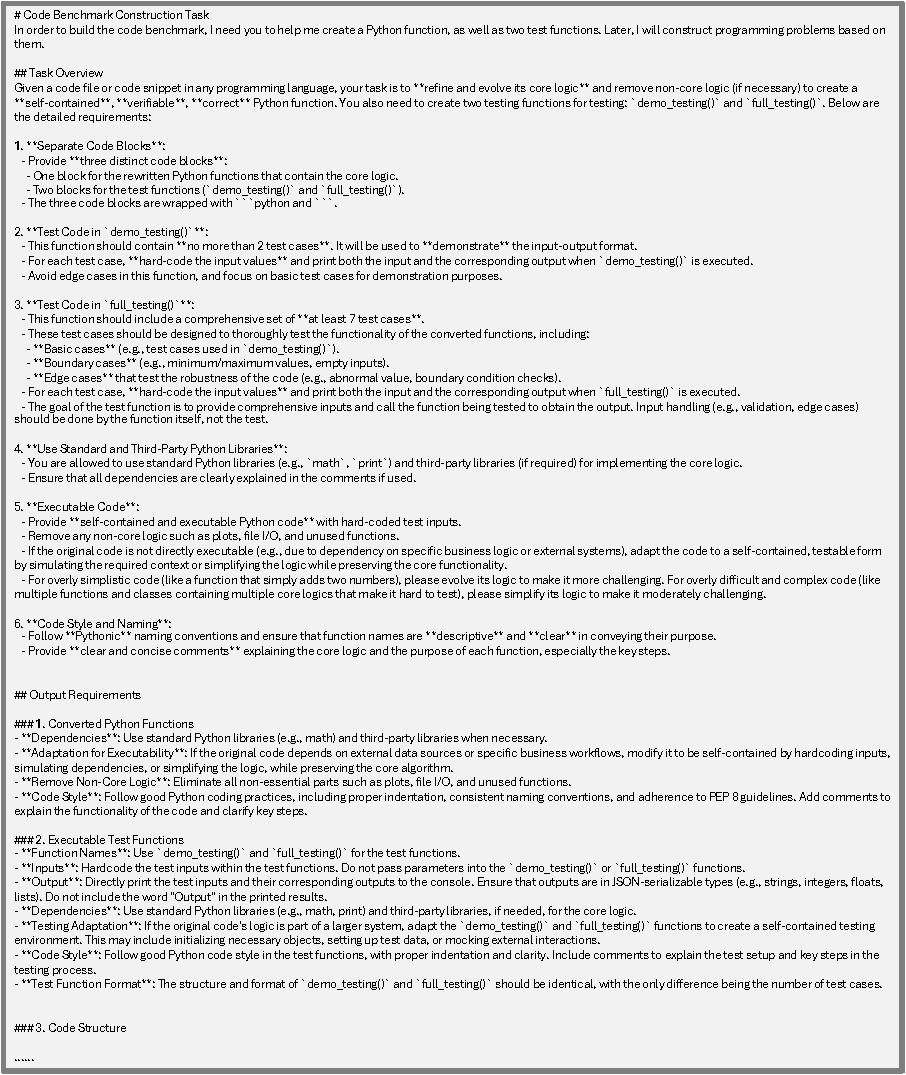
\includegraphics[width=0.9\textwidth]{figures/prompt_solution.pdf}
\caption{The prompt of generating code solution. Due to the excessive length of the prompt, we have omitted the latter part.}
\label{appendix:prompt_solution}
\end{figure}


\begin{figure}[t]
\centering
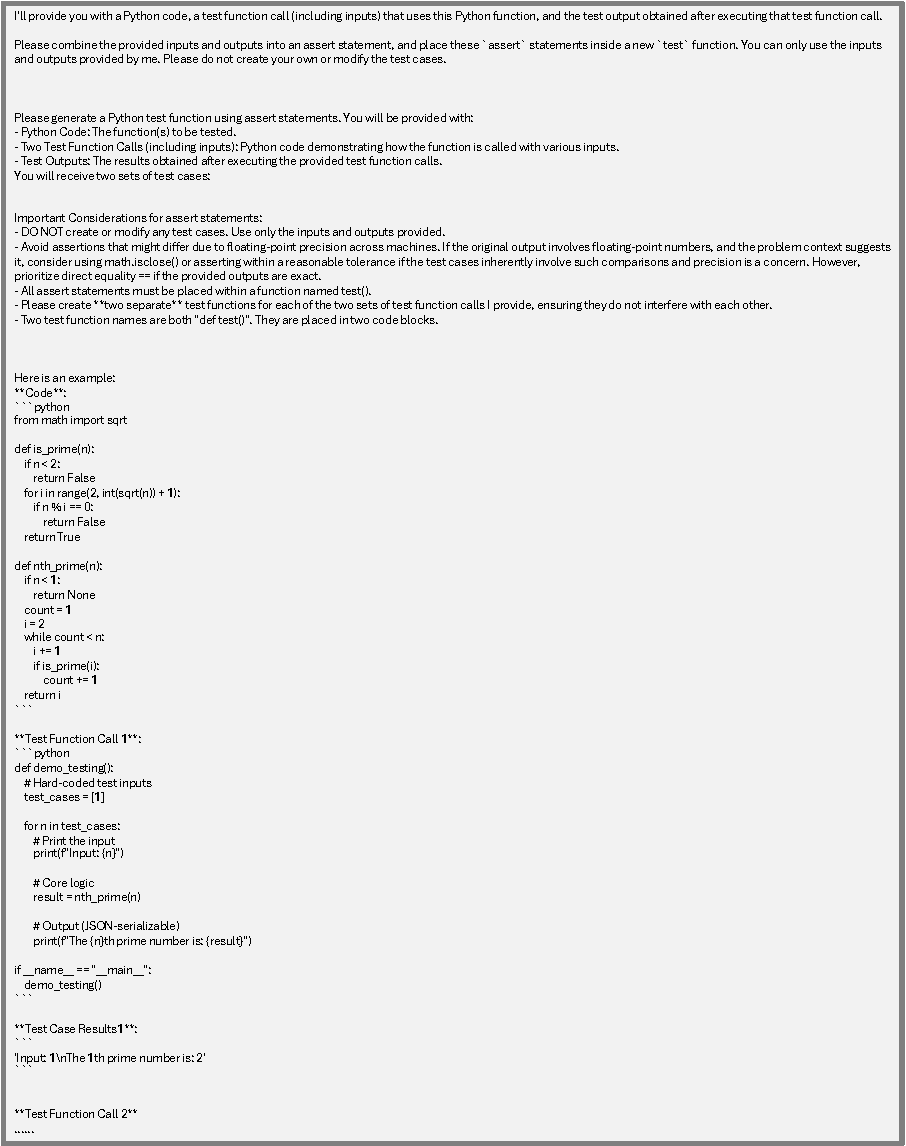
\includegraphics[width=0.9\textwidth]{figures/prompt_test.pdf}
\caption{The prompt of generating test function. Due to the excessive length of the prompt, we have omitted the latter part.}
\label{appendix:prompt_test}
\end{figure}

\begin{figure}[t]
\centering
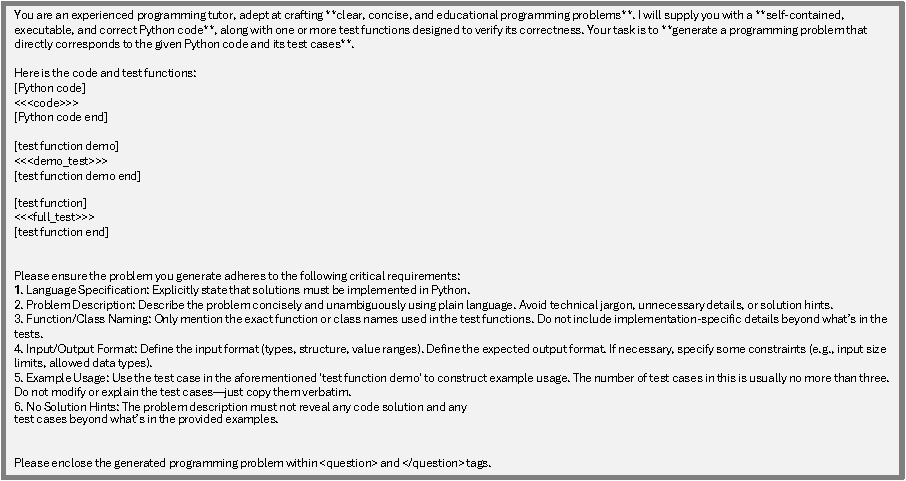
\includegraphics[width=0.9\textwidth]{figures/prompt_problem.pdf}
\caption{The prompt of generating programming problem.}
\label{appendix:prompt_problem}
\end{figure}



\begin{figure}[t]
\centering
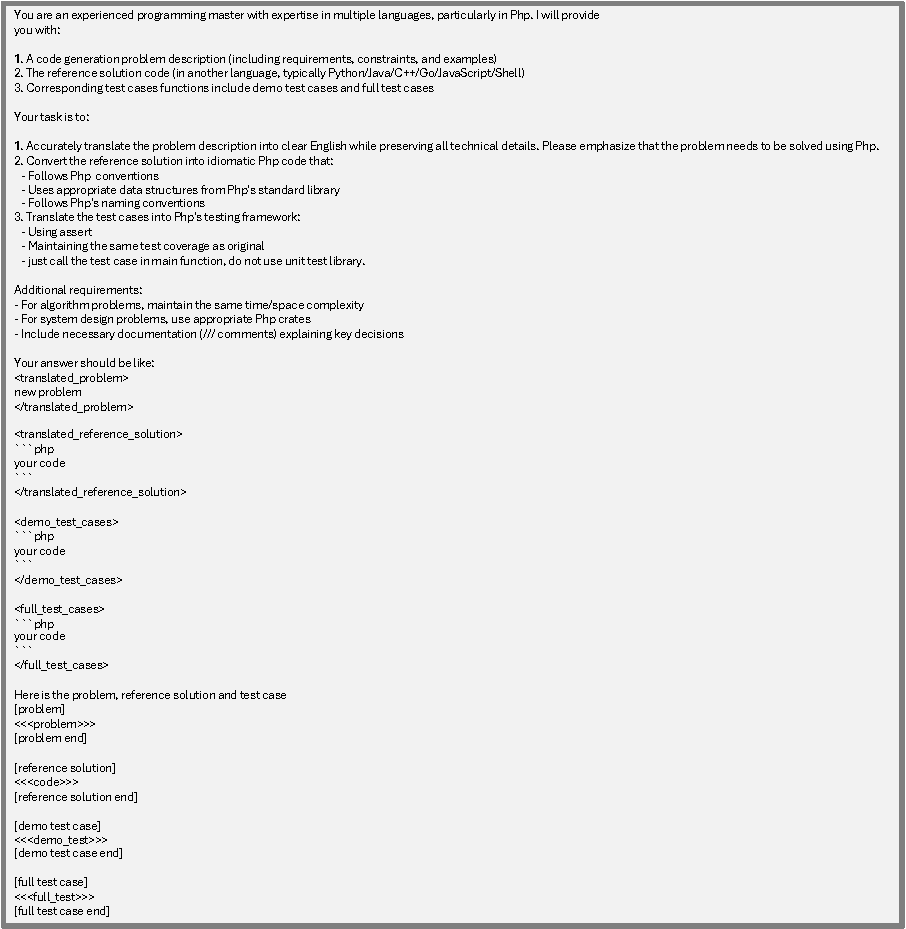
\includegraphics[width=0.9\textwidth]{figures/prompt_translate.pdf}
\caption{The prompt of translating languages.}
\label{appendix:prompt_translate}
\end{figure}